%% abtex2-modelo-include-comandos.tex, v-1.9.6 laurocesar
%% Copyright 2012-2016 by abnTeX2 group at http://www.abntex.net.br/
%%
%% This work may be distributed and/or modified under the
%% conditions of the LaTeX Project Public License, either version 1.3
%% of this license or (at your option) any later version.
%% The latest version of this license is in
%%   http://www.latex-project.org/lppl.txt
%% and version 1.3 or later is part of all distributions of LaTeX
%% version 2005/12/01 or later.
%%
%% This work has the LPPL maintenance status `maintained'.
%%
%% The Current Maintainer of this work is the abnTeX2 team, led
%% by Lauro César Araujo. Further $\infty$ormation are available on
%% http://www.abntex.net.br/
%%
%% This work consists of the files abntex2-modelo-include-comandos.tex
%% and abntex2-modelo-img-marca.pdf
%%

% ---
% Este capítulo, utilizado por diferentes exemplos do abnTeX2, ilustra o uso de
% comandos do abnTeX2 e de LaTeX.
% ---

\chapter{Uncertainty Quantification Background}\label{cap:background}


\begin{flushright}
	\textit{``UQ cannot tell you that your model is 'right' or 'true', \\
	but only that, if you accept the validity of the model (to some \\
	quantified degree), then you must logically accept the validity\\
	of certain conclusions (to some quantified degree)''\\
	\cite{Sullivan2015}}
\end{flushright}

Uncertainty Quantification (UQ) is a topic of great importance and hence widespread interest in computational analyses that are used to support important societal decisions on issues related to climate change \cite{allen2000quantifying, patt2005taking}, hurricane forecasts \cite{Tobergte2013}, subsurface hydrology \cite{Baroni2014a}, geology \cite{Guerra2016}, reactor safety [20-26], radioactive waste disposal [27-34], nuclear weapon safety [35-38], financial portfolios \cite{Chen2008}, environmental degradation [44- 47], and many additional areas of concern and challenge.

In this Chapter, we review the UQ specialized literature, comment some interesting results and highlight the challenges we are interested in the present thesis. The rest of the Chapter is organized as follow: in Section \ref{sec:definitions} we define what we understand as uncertainty, the differences between uncertainties and errors, some classifications of the uncertainties, and finally what is uncertainty quantification. In Section \ref{sec:uncertainty_representation} we introduce the mathematical formalisms used to represent uncertainty. Section \ref{sec:uq_problems} presents the main problems that UQ covers. Next, in Section \ref{sec:methods_uq_propagation} the two principal \textit{forward propagation} methods are referenced. Section \ref{sec:uq_large_scale} reviews the UQ challenges when we are in the presence of large-scale spatio-temporal models; and finally Section \ref{sec:background_summary} summarizes the Chapter.

\section{Definitions}\label{sec:definitions}
\subsection{Errors vs Uncertainties}

The mismatch between the true physical phenomena and the prediction obtained by modeling and simulation (M\&S) process can arise from the mathematical representation of a real problem, a physical problem (are the values of the parameters a good representation of the reality?), a computational problem (translation of a mathematical formulation into a numerical algorithm and a computational code) \cite{Lavril2015}. Uncertainty and error can be considered as the broad categories  that  are  normally  associated to this mismatch. Until recently the terms uncertainty  and error  have  commonly  been  used  interchangeably.  It is believed, however, that failure to distinguish between these terms is detrimental to the quantification of credibility in M\&S. According to \cite{Alvin1998} we can classify errors and uncertainties as follow: 

\begin{itemize}
\item[•] \textbf{errors:} recognizable deficiencies of the model or the algorithms employed. Errors are associated to: physical approximations to simplify the modeling of a physical process, translation of the mathematical to computational model, numerical approximations (truncation or roundoff), etc. When the errors are known there are reasonable means of estimating its magnitude of the introduced error. 
\item[•] \textbf{uncertainties:} potential deficiency that is due to lack of knowledge. The different sources of uncertainty can be:
\begin{itemize}
\item[-] \textbf{parameter uncertainty}, which comes from the model parameters that are inputs to the computer model (mathematical model) but whose exact values are unknown to experimentalists and cannot be controlled in physical experiments, or whose values cannot be exactly inferred by statistical methods. Examples are the local free-fall acceleration in a falling object experiment, various material properties in a finite element analysis for engineering, and multiplier uncertainty in the context of macroeconomic policy optimization \cite{Kennedy2001}.
\item[-] \textbf{model inadequacy}, no model is perfect. Even if there is no parameter uncertainty, so that we know the true values of all the inputs required to make a particular prediction of the process being modeled, the predicted value will not equal the true value of the process. This discrepancy is considered as model inadequacy. Since the real process may itself exhibit random variability, we define model inadequacy to be the difference between the true mean value of the real world process and the code output at the true values of the inputs.
\item[-] \textbf{parametric variability}, which comes from the variability of input variables of the model. For example, the dimensions of a work piece in a process of manufacture may not be exactly as designed and instructed, which would cause variability in its performance. 
\item[-] \textbf{structural uncertainty}, aka model inadequacy, model bias, or model discrepancy, which comes from the lack of knowledge of the underlying true physics. It depends on how accurately a mathematical model describes the true system for a real-life situation, considering the fact that models are almost always only approximations to reality. One example is when modeling the process of a falling object using the free-fall model; the model itself is inaccurate since there always exists air friction. In this case, even if there is no unknown parameter in the model, a discrepancy is still expected between the model and true physics. 
\item[-] \textbf{algorithmic uncertainty}, aka numerical uncertainty, which comes from numerical errors and numerical approximations per implementation of the computer model. Most models are too complicated to solve exactly. For example, the finite element method or finite difference method may be used to approximate the solution of a partial differential equation, which, however, introduces numerical errors. Other examples are numerical integration and infinite sum truncation that are necessary approximations in numerical implementation. 
\item[-] \textbf{experimental uncertainty}, aka observation error, which comes from the variability of experimental measurements. The experimental uncertainty is inevitable and can be noticed by repeating a measurement for many times using exactly the same settings for all inputs/variables. 
\item[-] \textbf{interpolation uncertainty}, which comes from a lack of available data collected from computer model simulations and/or experimental measurements. For other input settings that don't have simulation data or experimental measurements, one must interpolate or extrapolate in order to predict the corresponding responses.
\end{itemize}
\end{itemize}

A more elegant definition of what uncertainty is, is enunciated in \cite{Helton2009} as:

\begin{defn}
Uncertainty is a best estimate of the range of a particular metric which may derive from one or two broad sources. Uncertainties that reflect a lack of knowledge about the appropriate value to use for a quantity that is assumed to have (missing modifier: a fixed?) value in the context of a particular analysis are termed \textbf{\textit{epistemic}}. Uncertainties that arise from an inherent randomness in the behavior of the system under study are termed \textbf{\textit{aleatoric}}.
\end{defn}

\subsection{Aleatoric vs Epistemic Uncertainty}

It is sometimes assumed that uncertainty can be classified into those two categories, \textbf{\textit{aleatoric}} and \textbf{\textit{epistemic}}, although the validity of this categorization is open to debate \cite{Kiureghian2009}. 

\textbf{Aleatoric uncertainty} arises from an inherent randomness in the properties or behavior of the system under study. For example, the weather conditions at the time of a reactor accident are inherently random with respect to our ability to predict the future. Other examples include the variability in the properties of a population of weapon components and the variability in the possible future environmental conditions that a weapon component could be exposed to. Alternative designations for \textbf{aleatory uncertainty} include variability, stochastic, irreducible and type A. \cite{Helton2009}

\textbf{Epistemic uncertainty} derives from a lack of knowledge about the appropriate value to use for a quantity that is assumed to have a fixed value in the context of a particular analysis. For example, the pressure at which a given reactor containment would fail for a specified set of pressurization conditions is fixed but not amenable to being unambiguously defined. Other examples include minimum voltage required for the operation of a system and the maximum temperature that a system can withstand before failing. Alternative designations for \textbf{epistemic uncertainty} include state of knowledge, subjective, reducible and type B. \cite{Helton2009}

While \textbf{epistemic uncertainty} can be reduced through experiments, improvement of the numerical methods and so on, \textbf{aleatory uncertainty} can not be reduced. 


\subsection{Uncertainty Quantification}

UQ is not a mature field like linear algebra or single-variable complex analysis, with stately textbooks containing well-polished presentations of classical theorems. Both because of its youth as a field and its very close engagement with applications, UQ is much more about problems, methods and ‘good enough for the job’. There are some very elegant approaches within UQ, but as yet no single, general, overarching theory \cite{Sullivan2015}.

UQ neither have a unique and globally accepted definition. In the reviewed literature we find some definitions that, from our point of view, are those that better describe what UQ is.  

In the Wikipedia we find the following definition: 

\begin{defn}
Uncertainty Quantification is the science of quantitative characterization and reduction of uncertainties in applications. It tries to determine how likely certain outcomes are if some aspects of the system are not exactly known.
\end{defn}

This definition is very general and may ignore some important aspects, but as a first approach is a good one. 

In October of 2009 the U.S. Department of Energy organized a comission to study the impact of Extreme Scale computing in its National Security. One of the aspects analysed by the comission was UQ. In the report \textit{"Scientific Grand Challenges in National Security: The Role of Computing at the Extreme Scale"} \cite{DEnergy2009}, the authors define UQ as:

\begin{defn}
UQ studies all sources of error and uncertainty, including the following: systematic and stochastic measurement error; ignorance; limitations of theoretical models; limitations of numerical representations of those models; limitations of the accuracy and reliability of computations, approximations, and algorithms; and human error. A more precise definition is "UQ is the end-to-end  study of the reliability of scientific inferences". \cite{DEnergy2009}
\end{defn}

A more recent definition was introduced by Higdon et al. \cite{Higdon2017} in the \textit{"Handbook of Uncertainty Quantification"}:

\begin{defn}
UQ is the rational process by which proximity between predictions and observations is characterized. It can be thought of as the task of determining appropriate uncertainties associated with model-based predictions. More broadly, it is a field that combines concepts from applied mathematics, engineering, computational science, and statistics, producing methodology, tools, and research to connect computational models to the actual physical systems they simulate. In this broader interpretation, UQ is relevant to a wide span of investigations. These range from seeking detailed quantitative predictions for a well-understood and accurately modeled engineering systems to exploratory investigations focused on understanding trade-offs in a new or even hypothetical physical system. \cite{Higdon2017}
\end{defn}

Just to remark, in this definition the sentence: \textbf{a field that combines concepts from applied mathematics, engineering, computational science, and statistics, producing methodology, tools, and research to connect computational models to the actual physical systems they simulate}, illustrates the multidisciplinar nature of UQ and the main objectives of this research field.


\section{Uncertainty Representation}\label{sec:uncertainty_representation}

An immediate challenge in the development of an appropriate treatment of uncertainty is the selection of a mathematical structure to be used in its representation \cite{Helton2010}. Traditionally, probability theory has provided this structure. However, in the last several decades, additional mathematical structures for the representation of uncertainty such as evidence theory, possibility theory, fuzzy set theory, and interval analysis have been introduced.
This introduction has been accompanied by a lively discussion of the strengths and weaknesses of the various mathematical structures for the representation of uncertainty. For perspective, several comparative discussions of these different approaches to the representation of uncertainty are available.

%\cite{Helton2010a}

This section briefly summarizes some of this approaches, and discuss in more details probability theory as this is the main one used in the rest of the thesis.

\subsection{Interval Analysis}
Interval analysis is the simplest way to represent the uncertainty used when nothing more can be said about some unknown quantity than a range of it possible values. All the values have the same probability. For example, in the case of some unknown variable $x$, such information may be expressed as: $x \in [a, b]$, where $a$ and $b$ represent the left and right limit of the interval. This is a very basic form of uncertainty \cite{Sullivan2015}.

\subsection{Variance}
Suppose that, for a random variable $X \in \mathcal{X}$, the knowledge is summarized by a probability function $p \in P(\mathcal{X})$. The probability measure $p$ is a very rich and high-dimensional object, but sometimes we need to summarize the uncertainty in $p$, with just one number. Variance is an obvious statistic to summarize this. The formal definition of Variance is:

\begin{defn}
Variance is the expectation of the squared deviation of a random variable from its mean. The variance measures how far each number in the set is from the mean.
\end{defn}

If we know the mean $m$ of $p$, then the Variance can be computed as:

\begin{equation}
\mathcal{V}(\textit{p}) = \int_{\mathcal{X}} \|x-m\|^2dp(x) = E_{X~p}[\|X-m\|^2]
\end{equation}

If $\mathcal{V}(\textit{p})$ is small, then we are \textbf{relatively certain} that the values of $X$ are quite close to the mean $m$, and if $\mathcal{V}(\textit{p})$ is large, then we are more uncertain about $X$.

Variance and standard deviation $\sigma = \sqrt{\mathcal{V}(\textit{p})}$ are the standard way of quantify the uncertainty of a random variable. This is due to its simplicity of interpretation and easy to compute. But, there are some interesting questions that arise in UQ context that can't be answered correctly by the use of low order statistical moments, as Lampasi et al. \cite{Lampasi2006} say, only assessing the complete PDF allow aware decisions. 

It is clear that assessing the complete PDF of each random variables at each spatio-temporal location, and worse yet, when we are in the presence of large-scale models, is a computational intensive task. But, this is exactly the main objective of this thesis, to present a new workflow to compute the PDF at each spatio-temporal location, and demonstrate its practical use answering the research questions enunciated in Chapter \ref{cap:intro}.

\subsection{Information Entropy}
\label{InformationEntropy}
The concept of information entropy was first defined by Shannon (1948) in a study performed to identify the amount of information required to transmit English text. The underlying idea was that, given the probabilities of letters occurring in the English alphabet, it is possible to derive a measure describing the missing information to determine the full text of a partially transmitted message, where information is understood as the one required to identify the message, not the information of the message itself. Based on several theoretical considerations, Shannon derived the following equation to classify a measure of the missing information, often referred to as information entropy:

\begin{equation}
H=-\sum_{i}^N p_{i}\log p_{i}
\end{equation}

The information entropy \textit{H} is defined as the sum of the product of the probability \textit{p} for each possible outcome \textit{i} of \textit{N}, total possible outcomes, with its logarithm. The minimum value is 0, because $\log 1=0$. 

\subsubsection{Information entropy in a spatio-temporal context}
\label{InformationEntropySpatioTemporal}
For each spatio-temporal region, the information entropy can be described as: 

\begin{equation}\label{eq: spatio-temporal Entropy}
H(s,t)=-\sum_{m=1}^M p_{m}(s,t)\log p_{m}(s,t)
\end{equation}
where $s$ denotes the location of the subregion, $M$ represents the number of possible (exclusive) members the subregion may contain, and $t$ is the physical time.

\subsubsection{Information entropy as a meause of uncertainty}\label{subsub:informationentropytomeasuretheuncertainty}
Based on \ref{InformationEntropy} and \ref{InformationEntropySpatioTemporal}, if the possible outcomes of the model and the probability of each outcome on each $(s,t)$, are known, then the information entropy could be used as a qualitative measure of the uncertainty of the model output \cite{Wellmann2012}. For example, in a spatio-temporal region $(s,t)$ where the outcome is always the same, the information entropy is 0, because the outcome is known. On the other hand, in the worse case where all the outcomes have the same probability in $(s,t)$, the entropy is maximum and the uncertainty too.

%The main limitations of this method, is that the possible outcomes of the model are  usually not known. To tackle this problem, in section \ref{Clusterizing the GLD based in its lambda values} we present a novel algorithm that uses a clusterization method over the $\lambda$ values of the \textit{GLD}, to group the model output in possible outcomes. Then, with those outcomes we can apply Information Entropy to estimate the uncertainty on different contexts.

\subsection{Probability Theory}
Probability theory is based on the specification of a triple $(\Omega,\mathcal{F},P)$, where $\Omega$ is the set of all possible outcomes, $\mathcal{F}$  is a suitably restricted collection of subsets of $\Omega$, and $P$ defines the probability of the elements of $\Omega$.

The probability measure $P$ is a function returning an event's probability, with the properties that $0 \leq P \leq 1$ and $P(\Omega)=1$

One way to characterize the probability is through the probability density function (\textit{PDF}). It is a mathematical function that, stated in simple terms, can be thought of as providing the probabilities of occurrence of different possible outcomes in an experiment. 

\textbf{Probability density function}: for a continuous random variable $X$, we can define the probability that $X$ is in $[a,b]$ as:
\begin{equation}
P(a<=X<=b)=\int_a^b f(x)dx
\end{equation}

where $f(x)$ is a probability density function, which satisfies two properties:
\begin{equation*}
\begin{aligned}
& f(x)>=0 \\ 
& \int_{-\infty}^{+\infty}f(x) dx =1
\end{aligned}
\end{equation*}
a, b are real numbers.
The \textit{PDF} defines the probability that $X<=a$ as
$P(X<=a)=\int_{-\infty}^a f(x) dx$

\section{Some Typical UQ Problems}\label{sec:uq_problems}
Many typical UQ problems can be illustrated in the context of a system $F$, that maps input $X$ in some space $\mathcal{X}$ to outputs $Y = \mathcal{M}(X)$ in some space $\mathcal{Y}$, through a mathematical/computational model $\mathcal{M}$. Some common UQ objectives include: \textit{forward propagation or push-forward problem}, Section \ref{seq:forward}; \textit{reliability or certification problem}, Section \ref{seq:reliability}; \textit{prediction problem}, Section \ref{seq:prediction}; \textit{inverse problem}, Section \ref{seq:inverse}; \textit{sensitivity analysis}, Section \ref{seq:sensitivity}; and \textit{model reduction or model calibration problem}, Section \ref{seq:calibration}. Roughly all of this objectives are summarized in Figure \ref{fig:uqlab_workflow}.

\begin{figure}[H]
    \centering
    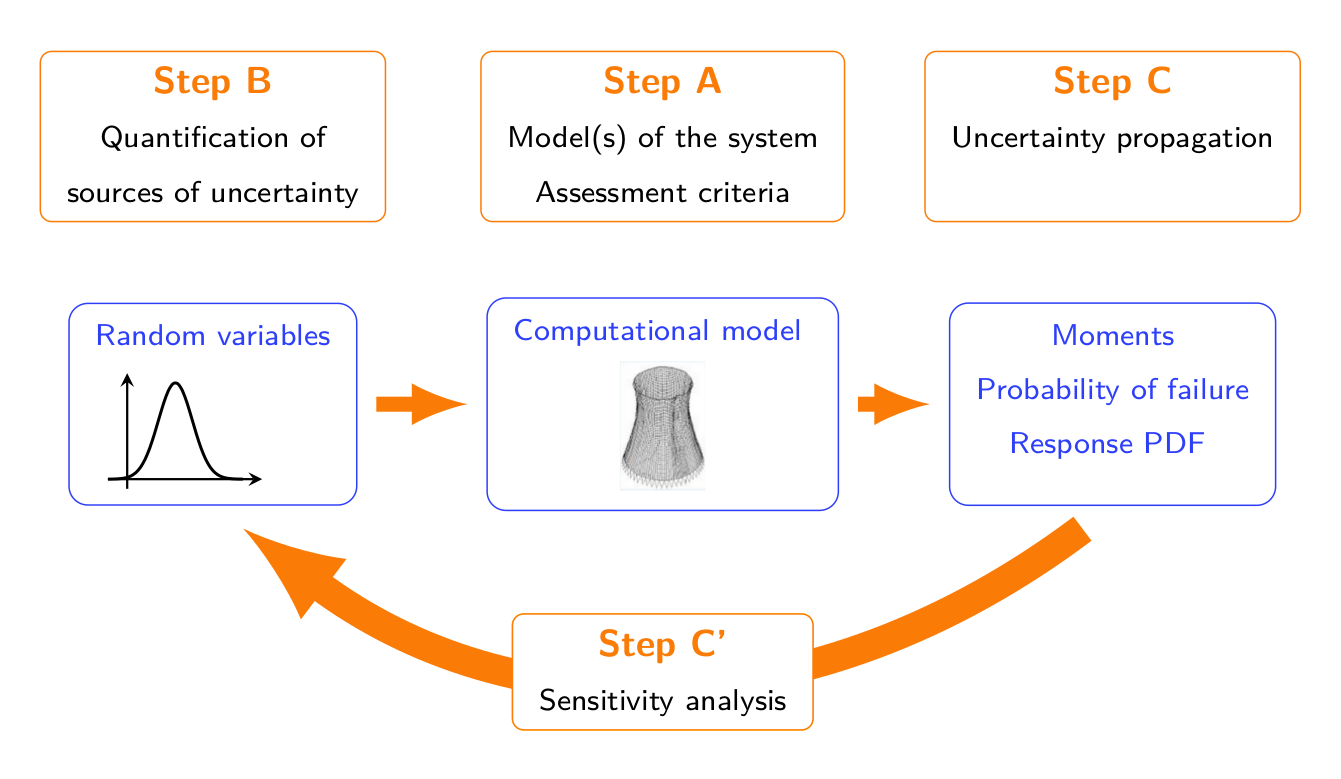
\includegraphics[width=0.8\textwidth]{img/background/UQ_steps.png}
    \caption{Uncertainty Quantification workflow. Taken from \href{http://www.uqlab.com/}{UQLab}.}
    \label{fig:uqlab_workflow}
\end{figure}

\subsection{Forward propagation or push-forward problem}\label{seq:forward}
Given the equation $\bm{Y}=\mathcal{M}(\bm{X})$ where: 
\begin{itemize}
\item $\bm{X} \in \mathcal{X} $ is a vector of  input parameters of the model,
\item $\mathcal{M}$ is a computational model, and
\item $\bm{Y} \in \mathcal{Y}$ is a vector that represents  quantities of interest (\textit{QoI}).
\end{itemize}
Suppose that the uncertainty about the inputs of $\mathcal{M}$ can be summarized in a probability distribution $P$ on $\mathcal{X}$. Then in a \textit{forward propagation}, the objective is to quantify the uncertainty of $\bm{Y}$, induced by $\bm{X}$ through $\mathcal{M}$.

The main objective of this thesis is a new method to quantify the uncertainty of the output of large-scale spatio-temporal models, that is a \textit{forward propagation problem}. In Section \ref{sec:methods_uq_propagation} some methods for \textit{forward propagation} are exposed; while in Section \ref{sec:uq_large_scale} we discus about \textit{forward propagation} in large-scale spatio-temporal models.  

\subsection{Reliability or certification problem}\label{seq:reliability}
Suppose that some set $\mathcal{Y}_{fail}\subseteq \mathcal{Y}$ is identified as a 'failure set'. Then in a reliability analysis we are interesting in, given appropriate information about the input $X$ and a process $F$, determine the failure probability 
\begin{equation}
\mathcal{P}[\mathcal{M}(X)\in \mathcal{Y}_{fail}]
\end{equation}
Furthermore, how large will the deviation from acceptable performance be, and what are the consequences? \cite{Sullivan2015}

\subsection{Prediction problem}\label{seq:prediction}
Similar to the reliability problem, given a maximum acceptable probability error $\epsilon > 0$, find a set $\mathcal{Y}_{\epsilon}\subseteq \mathcal{Y}$ such that
\begin{equation}
\mathcal{P}[\mathcal{M}(X)\in \mathcal{Y}_{\epsilon}]\geq 1-\epsilon
\end{equation}

in other works, the prediction $\mathcal{M}(X)\in \mathcal{Y}_{\epsilon}$ is wrong with probability at most $\epsilon$.

\subsection{Inverse problem or parameter estimation}\label{seq:inverse}
Given some experimental measurements of the output $Y$ of the system and some computer simulation results from its mathematical model $\mathcal{M}$, inverse uncertainty quantification estimates the discrepancy between the experiment and the mathematical model (which is called \textit{bias correction}), and estimates the values of unknown parameters in the model if there are any (which is called \textit{parameter calibration}) \cite{GharibShirangi2014}. Generally this is a much more difficult problem than forward uncertainty propagation; however it is of great importance since it is typically implemented in a model updating process.

\subsection{Sensitivity Analysis}\label{seq:sensitivity}
Sensitivity analysis refers to the determination of the contributions of individual uncertain analysis inputs to the uncertainty in analysis results. The goal in sensitivity analysis is to apportion the uncertainty in $Y$ to the uncertainty in inputs $X$, \cite{Sankararaman2012}. 

\subsection{Model reduction or model calibration problem}\label{seq:calibration}
Construct another model $\mathcal{M}_{h}$ such that $\mathcal{M}_{h} \approx \mathcal{M}$ in an appropriate sense. 

\subsection{Model selection}
If, for the system $F$ we have a set of models $\mathcal{M} = \lbrace \mathcal{M}_{1}, \mathcal{M}_{2},...,\mathcal{M}_{n} \rbrace$, then a model selection problem consist in the selection of the most plausible model $\mathcal{M}_{i}$ that best fits the experimental data.

Sometimes a UQ problem consists of several of these problems coupled together, for example, one might have to solve an \textbf{\textit{inverse problem}} to produce or improve some model parameters, and then use those parameters to propagate some other uncertainties \textbf{\textit{forwards}}, and hence produce a \textbf{\textit{prediction}} that can be used for decision support in some \textbf{\textit{certification problem}} \cite{Sullivan2015}.

In this thesis we focus on \textbf{\textit{forward propagation problem}} although in chapter \ref{cap:use_cases} we introduce some queries that help to solve \textbf{\textit{reliability or certification}} and \textbf{\textit{prediction problem}}.

\section{Methods for Forward Propagation}\label{sec:methods_uq_propagation}

Two different methods are used to study how the uncertainty is propagated through a computational model, \textit{intrusive} and \textit{non-intrusive}. \textit{Intrusive methods} require the modification of the mathematical/computational model. On the other hand, \textit{non-intrusive methods} consider the mathematical/computational model as a black-box, and therefore the simulation codes don't need to be rewritten. For this reason, non-intrusive methods are attractive \cite{Kawai2014}. The most popular methods for non-intrusive uncertainty propagation are sampling methods, such as Monte Carlo (\textit{MC}) and Latin hypercube sampling (\textit{LHS}). To date, the MC simulation is the most powerful method for the uncertainty propagation, \cite{Rajan2016}.

In this thesis we are not interested into the methods themselves because our principal objective is to process the uncertainty data generated as an output of a forward propagation process. To illustrate in a better way the problem, lets consider a \textit{non-intrusive method} as an example.

To estimate a stochastic behavior of the output solution $\bm{q}$  in terms of input uncertainties $\bm{\theta}$, the sampling methods analyze the values of $\mathcal{M}(\bm{\theta})$ at multiple sampled conditions in the $\Theta$ space (called stochastic space or parameters space) directly from numerical simulations. Basically, \textit{MC} and \textit{LHS} methods randomly sample in the stochastic space, and hence both require many sample calculations to achieve a convergence of stochastic estimations (although the \textit{LHS} method is more efficient than the \textit{MC} method). As a result, the method returns multiple realizations of $\bm{q}$, and then other methods to measure the uncertainty, as those proposed in Section \ref{sec:uncertainty_representation}, need to be applied,  \cite{Baxter2016, Estacio-Hiroms2012, Farrell2015}. 

The choise of one method to measure the uncertainty or other depends on the characteristics of each problem and the accuracy we are interesting in. But, as all results of interest can be derived from the \textbf{PDF} \cite{Cox2012}, our objective in this thesis is to use \textbf{PDFs} as the representation of the uncertainty. 
 
%In summary, in a \textit{forward problem}, there is  a computational model and, given a set of realization of the input random vector we are interested in capturing  the uncertainty at the \textit{QoI} $\bm{q}$. 

%\subsection{Monte Carlo}
%Monte Carlo simulations (MCS) consist of:
%\begin{itemize}
%\item[(i)] generating multiple realizations of the input parameters $\bm{\theta}$
%\item[(ii)] solving the deterministic model $\mathcal{M}(\bm{\theta})$ for each realization
%\item[(iii)] evaluating ensemble statistics or PDFs of these solutions
%\end{itemize}
%
%MCS do not impose limitations on statistical properties of input parameters, entail no modifications of existing deterministic solvers, and are ideal for parallel computing \cite{Higdon2017}.

Derive a PDF from uncertain data is a fitting process. Given a random sample $q_{1}, q_{2}, q_{3},...,q_{n}$, the basic problem in fitting a statistical distribution to these data is that of approximating the distribution from which the sample was obtained. 

Until now we review what uncertainty is, some definitions of uncertainty quantification, how to quantify the uncertainty, and some typical UQ problems. In the next section we explore what happens when we are in presence of a large-scale spatio-temporal model, which is the problem that really motivates this thesis.

\section{UQ in Large-scale Spatio-temporal models}\label{sec:uq_large_scale}
First to all lets define what is a large-scale spatio-temporal model (\textbf{LSSTM}). Although it is an extremely used term in the area, we don't find any exact definition in the reviewed literature. According to the Cambridge Dictionary, the mean of large-scale is:

\begin{defn}
\textbf{Large-scale}: involving many people or things, or happening over a large area.
\end{defn}

In the simulation context \textbf{happening over a large area} is the most appropriated term. The spatio-temporal part of the concept is straightforward. Join both ideas the definition of a large-scale spatio-temporal model could be considered as:

\begin{defn}
\textbf{Large-scale spatio-temporal model}: a mathematical/computational model that study the spatio-temporal evolution of a physical system over a large area.
\end{defn}

In this context, a computational model of the form: $\bm{q}=\mathcal{M}(\bm{\theta})$ represents the spatio-temporal evolution of a complex systems, and the \textit{QoI} $\bm{q}$ can be represented as:  

\begin{equation} \label{eq:spatio_temporal}
\mathbf{Q} = (\mathbf{q}(s_{1},t_{1}),\mathbf{q}(s_{2},t_{2}),...,\mathbf{q}(s_{n},t_{n}))  
\end{equation}
where:
\begin{itemize}
\item $(s_{1},t_{1}),(s_{2},t_{2}),....,(s_{n},t_{n}) \in \mathcal{S} \times \mathcal{T}\subseteq\mathbb{R}^{3}\times\mathbb{R}$ represent a set of distinct spatio-temporal locations, and
\item $\mathbf{q}(s_{i},t_{j})$ represents a value of the \textit{QoI} at the spatio-temporal location $(s_{i},t_{j})$
\end{itemize}
Many \textit{QoI} can be analyzed, but for simplicity in this thesis we consider only one.

When dealing with \textbf{LSSTMs}, a huge amount of data is generated as a result of the simulation process. Indeed, at each spatio-temporal location $(s_{i},t_{j}) \in \mathcal{S} \times \mathcal{T}\subseteq\mathbb{R}^{3}\times\mathbb{R}$, usually more than $10^4$ simulations are performed. Then, the size of the output dataset is in the order of $N_{s}\times N_{t}\times N_{sim}$, where: $N_{s}$ is the number of spatial locations, $N_{t}$ is the number of time steps, and $N_{sim}$ is the number of simulations.  An example of the volume of data generated by these simulations is given in the first case study of the Chapter \ref{cap:use_cases}, where the output dataset is about 2.4 TB. From a computational point of view, this classifies \textit{forward propagation} as a data intensive problem.

This information can be modeled as:
\begin{equation}\label{eq:data_base_structure}
S(s_{i},t_{j},simId,q(s_{i},t_{j}))
\end{equation}
where $simId$ represents the \textit{id} of one simulation (realization).

The emerging field of data science, nevertheless, is largely lacking in generalizable methods for quantifying the uncertainty in the output of analyzed systems. As a result, a major new research initiative needs to be initiated in this area \cite{Tobergte2013}.

Remember, we are interested in characterizing the uncertainty at each spatio-temporal location through a PDF. If we know, by theoretical considerations, that the distribution at each location is of certain type (e.g. normal, gamma, beta), then through moment matching, one can determine a specific distribution that fits the data at that location, \cite{Karian2011, Mustafa2016}. This is usually not the case, even worse in \textbf{LSSTM}, because it is impossible to know what could be a distribution type at each location. In those cases it makes sense to use a flexible family of distributions and choose a specific member of that family.

By a \textbf{flexible family} we mean one whose members can:

\begin{itemize}
\item[(i)] assume a large variety of shapes: skewness in either direction, tails that are truncated or extend to infinity on either or both sides, bell-shaped distributions as well as inverted bell-shaped ones,
\item[(ii)] be able to represent a wide range of distributional characteristics such as moments (or combination of moments) or percentiles (or combinations of percentiles),
\item[(iii)] to have convenient expressions for at least one of their p.d.f., c.d.f., and quantile function,
\item[(iv)] no prior knowledge is needed to fit the distribution to a dataset, which is practical and suitable for automatic and software procedures.
\end{itemize} 

Another challenge that emerges from \textbf{LSSTM} is related to the amount of data. It is not always convenient to retain the $N_{s}\times N_{t}\times N_{sim}$, (vector) values produced by MC and use them subsequently \cite{Cox2012}. This fact introduces another desirable characteristic of the distribution family.

\begin{itemize}
\item[(v)] reduce the amount of data to use in subsequent UQ analysis, after the \textbf{PDF} is obtained. 
\end{itemize}

In Chapter \ref{cap:gld} we present one of this distribution families an discus why this family is suitable to our proposes. 
%The question of how to represent and communicate uncertainties is a topic of research both from a practical and theoretical point of view. A fair bit of theoretical research is aimed at the mathematical calculus of uncertainty. This includes extensions and alternatives to standard probabilistic reasoning, such as Dempster-Schafer theory and imprecise probabilities. When uncertainties are needed for investigations requiring computational models, additional considerations arise. For example, if the simulation output is a daily surface-temperature field over the globe for the next 200 years, representing uncertainty and dependencies is complex. Should ensembles be used to represent plausible outcomes? How should these ensembles of simulation output be stored? How can high-consequence/low-probability outcomes be discovered in this massive output? Here some research investigations attempt to leverage theory that exploits high dimensionality to bound probabilities and system behavior. Finally, even when uncertainties are well captured, how best to communicate such uncertainties to the public or to decision-makers is also a topic of ongoing research. 
%\cite{DEnergy2009}

%\section{Software and Tools for UQ}
%Currently, advances in uncertainty propagation and assessment have been paralleled by a growing number of software tools for uncertainty analysis, but none has gained recognition for a universal applicability, including case studies with spatial models and spatial model inputs. \cite{Sawicka2016}
%
%These include both free software, like OpenTURNS (Andrianov et al., 2007), DACOTA (Adams et al., 2009) and DUE (Brown and Heuvelink, 2007), commercial, like COSSAN (Schuëller and Pradlwarter, 2006), or free, but written for a licenced software, e.g. SAFE (Pianosi et al., 2015) or UQLab (Marelli and Sudret, 2014) toolboxes for MATLAB. A broad review of existing software packages is available in Bastin et al. (2013). To the best of our knowledge, however, none of the existent software is specifically designed to be extended by the environmental science community. The use of powerful but complex languages like C++ (e.g. Dakota), Python (e.g. OpenTURNS) or Java (e.g. DUE) often discourages relevant portions of the non-highly-IT trained scientific community from the adoption of otherwise powerful tools.
%spup-R package \cite{Sawicka2016}. De aqui saque lo de arriba tambien, aunque lo de arriba lo puedo buscar en sus respectivos papers y hablar un poco de cada uno de ellos.

\section{Summary}\label{sec:background_summary}

Summarizing, in this Chapter we present a review about UQ, showing what is uncertainty quantification; the principal mathematical tools used to represent it; and the typical UQ problems. Immediately we talk about some methods for uncertainty propagation and the problems we are interested in. Basically, we are interested in proposing a new Big Data approach that would allow to compute a \textbf{PDF} at each spatio-temporal location of the output of a forward propagation problem.


